\section{Auswertung}%
\label{sec:auswertung}

\subsection{Statische Bestimmung des Erdmagnetfeldes}%
\label{sub:statische_bestimmung_des_erdmagnetfeldes}

\begin{figure}[h]
	\centering
	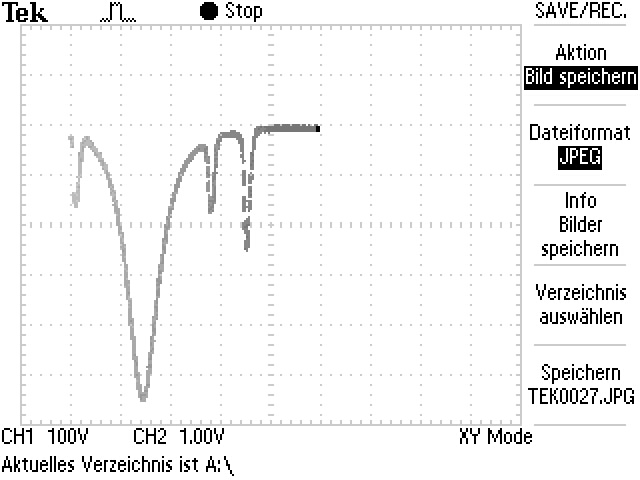
\includegraphics[width=0.8\linewidth]{picture/Transmission_Spek.JPG}
	\caption{}
	\label{fig:}
\end{figure}


\subsection{Landefaktoren der Rubidium Isotope}%
\label{sub:landefaktoren_der_rubidium_isotope}


\begin{table}[h]
	\centering
	\caption{caption}
	\label{tab:label}
	\sisetup{%
		round-mode=places,
		table-format=3.1,
		round-precision=1,
	}
		\input{build/b_nu.tex}
\end{table}

\begin{table}[h]
	\centering
	\caption{caption}
	\label{tab:label}
	\sisetup{%
		round-mode=figures,
		round-precision=3,
		table-format=1.2e3
	}
	\input{build/lin_params.tex}
\end{table}

\begin{figure}[h]
	\centering
	\includegraphics[width=0.8\linewidth]{build/static_B.pdf}
	\caption{Name}
	\label{fig:name}
\end{figure}

\subsection{Bestimmung der magnetischen Momente des Kerns}%
\label{sub:bestimmung_der_magnetischen_momente_des_kerns}

\begin{table}[h]
	\centering
	\caption{caption}
	\label{tab:label}
	\input{build/lande.tex}
\end{table}

\begin{table}[h]
	\centering
	\caption{Kernspins}
	\label{tab:label}
	\input{build/kernspin.tex}
\end{table}

\subsection{Bestimmung des Isotopenverhaeltniss}%
\label{sub:bestimmung_des_isotopenverhaeltniss}

\subsubsection{statisch}%
\label{ssub:statisch}

\begin{equation}
	\frac{A_{85}}{A_{87}} = ??
\end{equation}

\subsubsection{dynamisch}%
\label{ssub:dynamisch}


\begin{figure}[h]
	\centering
	\begin{subfigure}[c]{0.45\textwidth}
	\begin{center}
	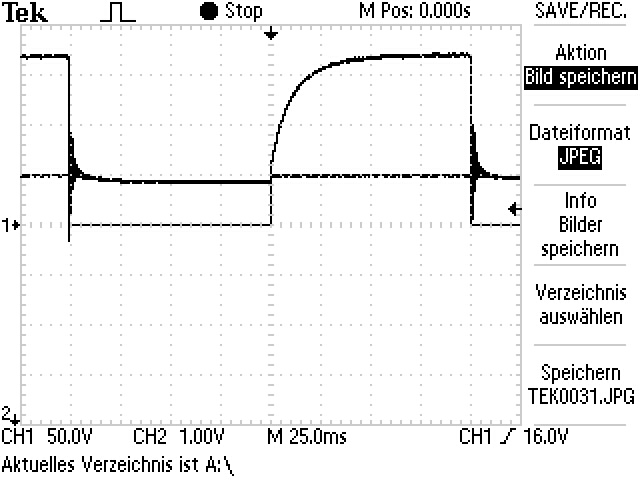
\includegraphics[width=\textwidth]{./picture/Peak_1.JPG}
	\end{center}
	\caption{Peak 1}
	\label{fig:}
	\end{subfigure}
	\begin{subfigure}[c]{0.45\textwidth}
	\begin{center}
	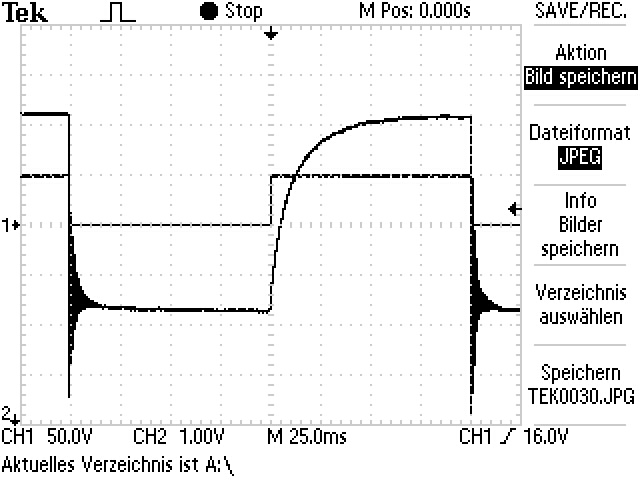
\includegraphics[width=\textwidth]{./picture/Peak_2.JPG}
	\end{center}
	\caption{Peak 2}
	\label{fig:}
	\end{subfigure}
	\caption{}
	\label{fig:}
\end{figure}

\begin{table}[h]
	\centering
	\caption{caption}
	\label{tab:label}
	\begin{subtable}[t]{0.4\textwidth}
	\centering
	\caption{caption}
		\input{build/T1.tex}
	\end{subtable}
	\begin{subtable}[t]{0.4\textwidth}
	\centering
	\caption{caption}
		\input{build/T2.tex}
	\end{subtable}
\end{table}

\begin{figure}[h]
	\centering
	\begin{subfigure}[c]{0.45\textwidth}
	\begin{center}
		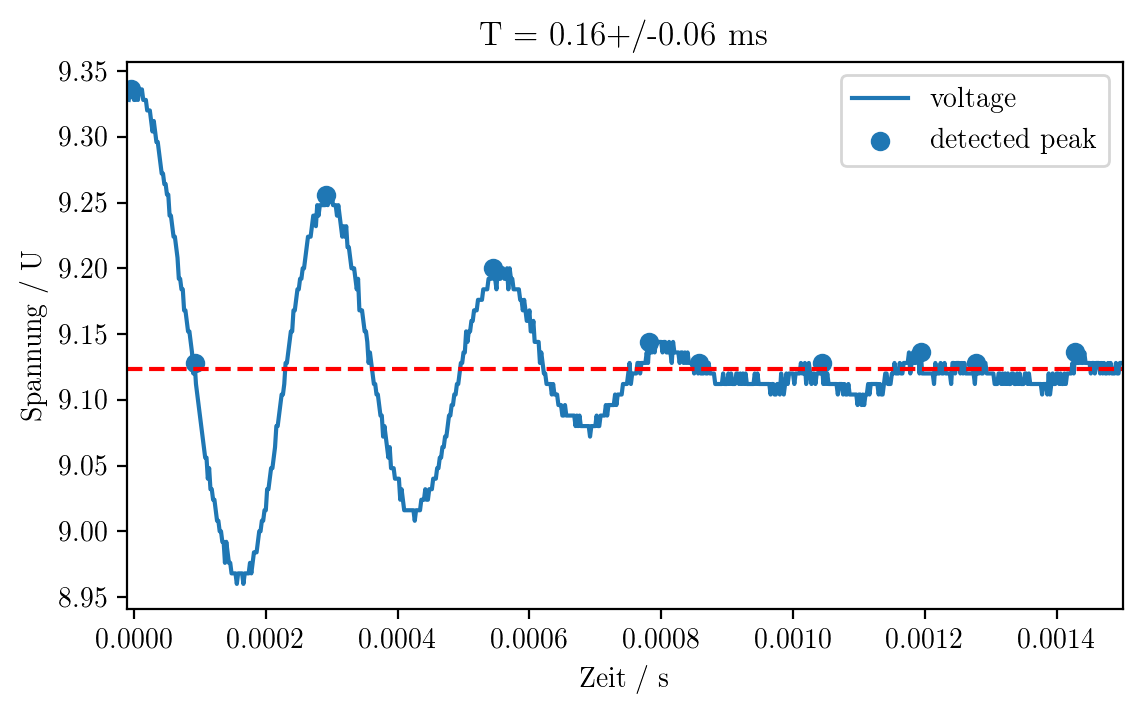
\includegraphics[width=\textwidth]{build/firstPeak_3.png}
	\end{center}
	\caption{}
	\label{fig:}
	\end{subfigure}
	\begin{subfigure}[c]{0.45\textwidth}
	\begin{center}
		\includegraphics[width=\textwidth]{build/firstPeak_9.png}
	\end{center}
	\caption{}
	\label{fig:}
	\end{subfigure}

	\begin{subfigure}[c]{0.45\textwidth}
	\begin{center}
		\includegraphics[width=\textwidth]{build/secondPeak_3.png}
	\end{center}
	\caption{}
	\label{fig:}
	\end{subfigure}
	\begin{subfigure}[c]{0.45\textwidth}
	\begin{center}
		\includegraphics[width=\textwidth]{build/secondPeak_9.png}
	\end{center}
	\caption{}
	\label{fig:}
	\end{subfigure}
	\caption{}
	\label{fig:}
\end{figure}
